\section{Data Processing}
\label{sec:data-processing}

\subsection{Trigger}
As described in section \ref{sec:dom-daq}, the high-frequency ATWD waveform digitization in each DOM is triggered when it and its adjacent or next-to-adjacent neighbors on the same string record a voltages of at least 0.25 PE-equivalent within a $\pm$1~$\mu$s time window, which is referred to as the Hard Local Coincidence (HLC) condition. Data acquisition for DeepCore is triggered when this condition is fulfilled for at least three DOMs inside the DeepCore fiducial volume within a $\pm$2.5~$\mu$s window. If this condition is met, the waveforms for all DOMs that have observed voltages of at least 0.25~PE within a $\pm$10~$\mu$s time window centered around the trigger time are recorded. A DOM that is included in this readout but for which the HLC condition has not been met is said to fulfill the \emph{Soft Local Coincidence} (SLC) condition. The DeepCore trigger rate is less than 10~Hz and will trigger on \~70\% of $\nu_\mu$ events at 10~GeV and >90\% of $\nu_\mu$ events at 100~GeV\cite{DeepCore}.

\subsection{Online Filter}

Once the trigger condition is met, the recorded waveforms within the trigger window are converted into reconstructed pulses and are then passed into a set of \emph{online} filters (i.e. filters running on hardware at the Pole). These filters are each designed to select events that are relevant to different physics measurements that are performed within the IceCube collaboration. For the purposes of the analysis presented in this thesis, events are selected using the \emph{DeepCore filter}. This filter is designed to select events that start inside the DeepCore fiducial volume and to reject those that are consistent with muons entering the detector from the outside.
\begin{marginfigure}
    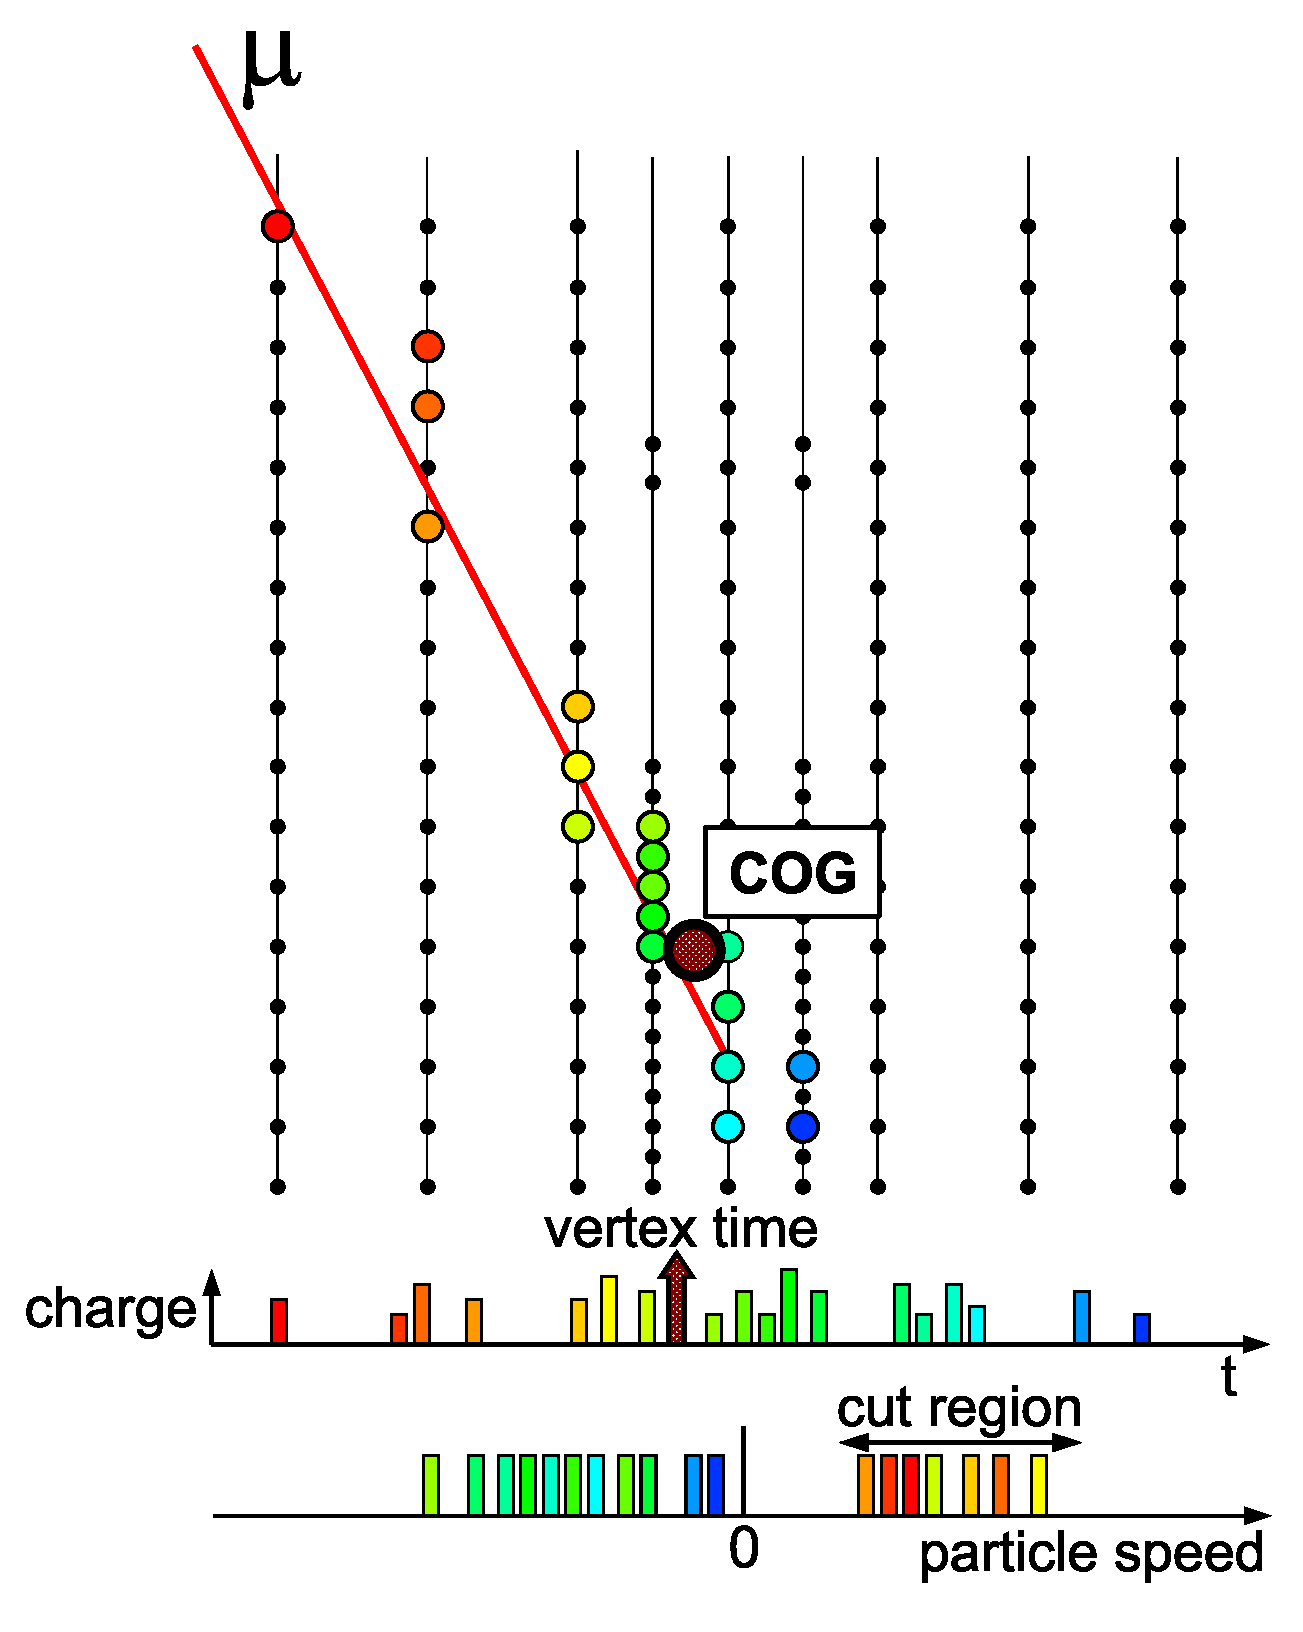
\includegraphics[width=\textwidth]{figures/icecube/eventviews/FilterDiagram.pdf}
    \caption{Example of an event that would be rejected by the online filter algorithm. DOMs that have observed light are highlighted in color depending on time from red (early hits) to blue (late hits). DOMs that have not observed any light are shown as black dots. Figure taken from \cite{DeepCore}.}
    \label{fig:online-filter-event}
\end{marginfigure}
The filter first applies a noise cleaning algorithm based on a coincidence condition between hits on different DOMs, where hits in DOMs for which the HLC condition was met are always kept. The cleaned hit series is split between those hits that fall within the DeepCore fiducial volume and those outside of it. The veto algorithm then calculates the COG in space and time of the hits inside the fiducial volume and then the velocity that a signal would have to travel from each hit occurring outside the fiducial volume to coincide with the COG. If this velocity is close to the speed of light (between $0.25\;\mathrm{ns/s}$ and $0.4\;\mathrm{ns/s}$) for at least one hit, the event is rejected because it is consistent with a muon traveling through the veto region and entering DeepCore. Figure~\ref{fig:online-filter-event} shows an example of an event that would be rejected by the online filter. Only events passing the trigger and filter condition are sent North via satellite for further \emph{offline} filtering.

\subsection{Offline Filter}

The offline filter is separated into subsequently applied \emph{levels}, referred to as L3, L4, and L5, where each level reduces the amount of background (atmospheric muons and noise) by approximately an order of magnitude while keeping most of the DeepCore starting events that are the target of the selection.

\subsubsection{Level 3}
At the lowest offline filter level, L3, cuts are applied to simple variables that remove the most easily identifiable background events while using only few computational resources. The variables aimed at cutting noise consist mostly of different DOM hit counts within hit series to which noise cleaning algorithms have been applied. The cuts aimed at removing muons consist of conditions on the number of hits in the veto region as well as conditions on the vertical position of the first HLC hit. The distribution for one of the variables used in the L3 filter is shown in figure~\ref{fig:l3-var-cleaned-full-time-length}. It is apparent from the distributions that there is a significant population of events in data with large values of the plotted variable that does not exist in simulation. These events are discarded, improving the agreement between data and simulation for events passing the L3 filter.
\begin{figure}
    \centering
    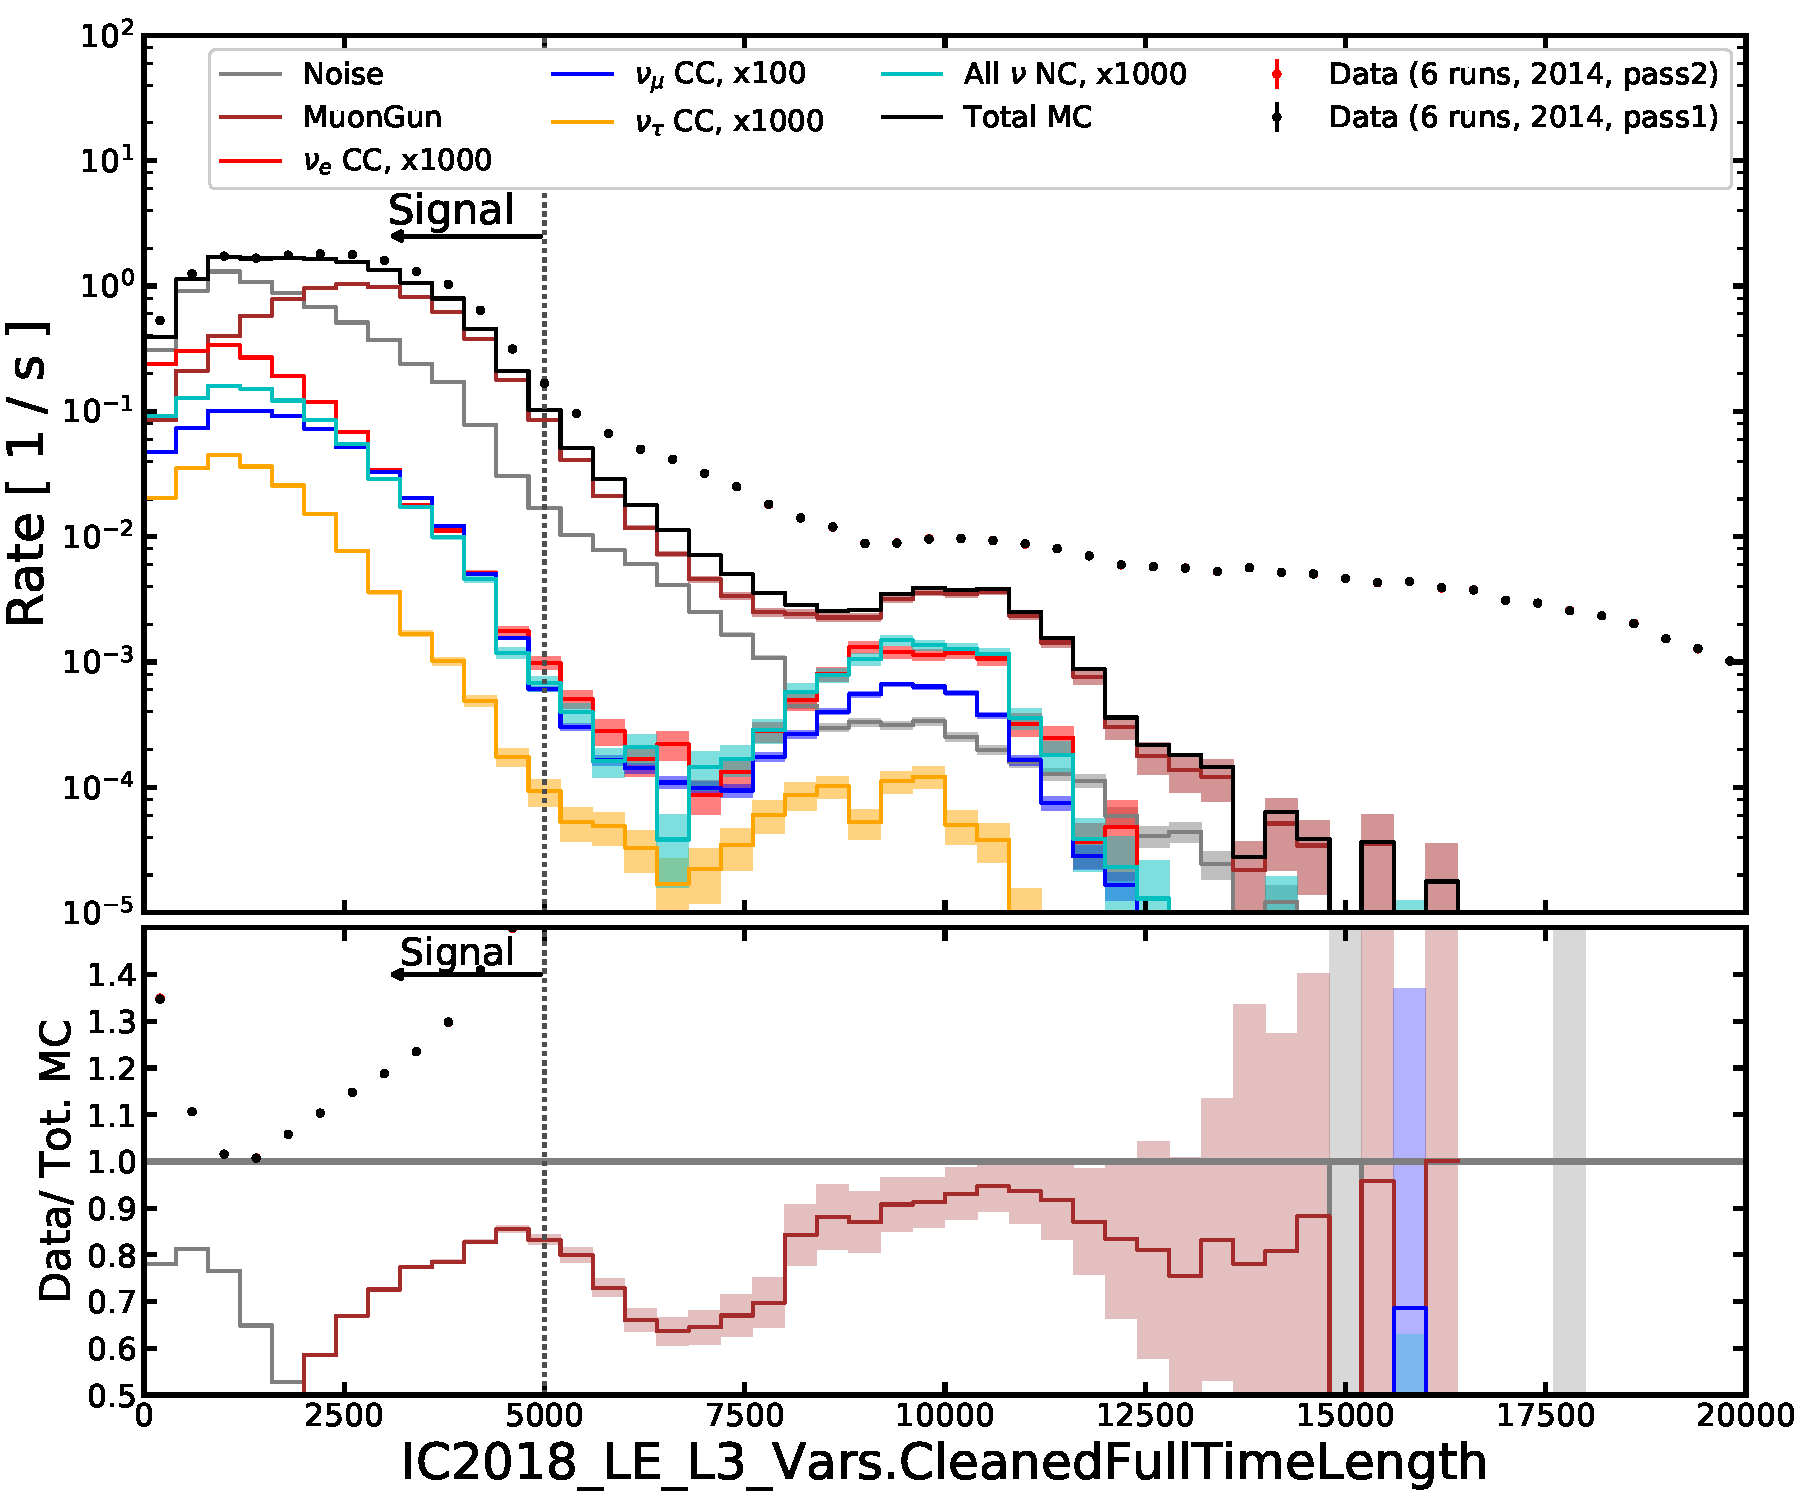
\includegraphics[width=7 cm]{figures/icecube/selection/IC2018_LE_L3_Vars_CleanedFullTimeLength.pdf}
    \caption{Distribution of one of the variables used in the L3 offline filter, the time between the last hit and the first hit after noise cleaning. Histograms show the distributions in simulated data separated by particle and interaction type, data points with error bars show the distribution of real data. The bottom panel shows the ratio between data and simulation. Events falling on the "signal" side of the histogram are passed to the next filter level.}
    \label{fig:l3-var-cleaned-full-time-length}
\end{figure}

\subsubsection{Level 4}
In the next level, L4, more advanced selections based on the output of Boosted Decision Trees (BDTs) are applied, with a separately trained BDT for noise and muon rejection, respectively. The output of each BDT is a probability score between zero (background-like) and one (signal-like).  The inputs into the BDT aimed at noise rejection consist of hit counts in cleaned hit series and variables that characterize the geometric and temporal spread of the observed hits, such as the full width half maximum (FWHM) of the hit times. The BDT is trained using simulated pure noise and neutrino events. Events are passing the L4 noise cut if the BDT score is above 0.7, which reduces the number of pure noise events by two orders of magnitude from 36.6~mHz to approximately 0.3~mHz. The BDT that is used to reject atmospheric muons also takes simple variables as its input that consist mostly of different veto hit counts and variables that characterize the distribution of z-coordinates of the observed hits as well as their radial distance with respect to the center of the DeepCore fiducial volume. In contrast to the noise BDT, however, the muon BDT is trained using real data and simulated neutrino events, with the goal of rejecting data events. This is possible because the data sample consists to 99\% of atmospheric muons at this stage of the event selection. Events are passing the L4 muon cut if the output score from the muon BDT is above 0.65, removing 94\% of all muon events while keeping 87\% of all neutrinos. The distributions of the output scores of both BDTs are shown in figure~\ref{fig:l4-bdt-output}.
\begin{figure*}
    \centering
    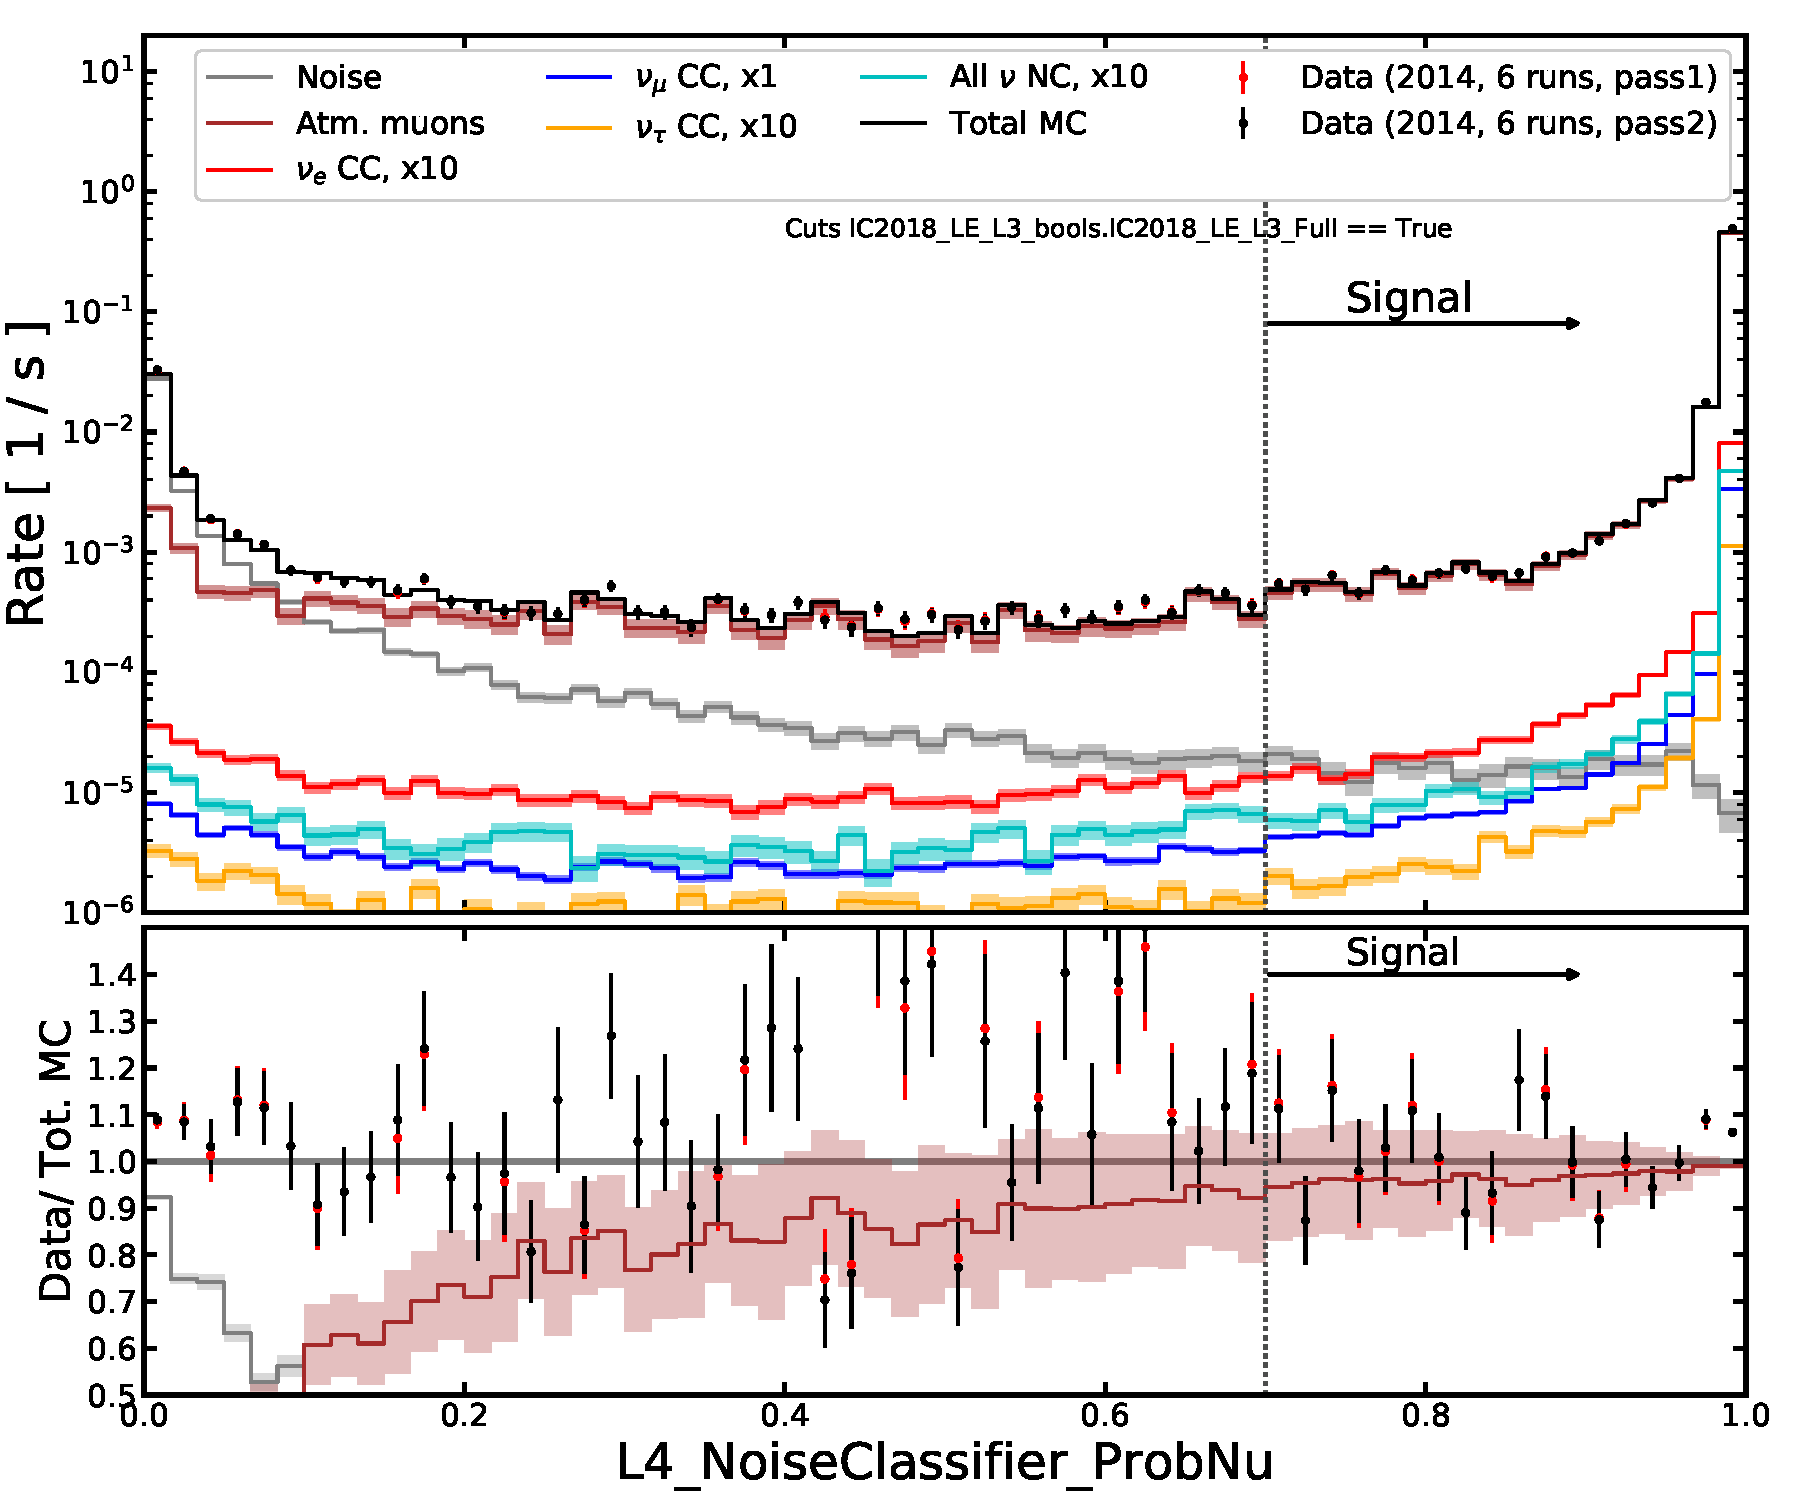
\includegraphics[width=7 cm]{figures/icecube/selection/L4_noiseBDT_L4_NoiseClassifier_ProbNu.pdf}
    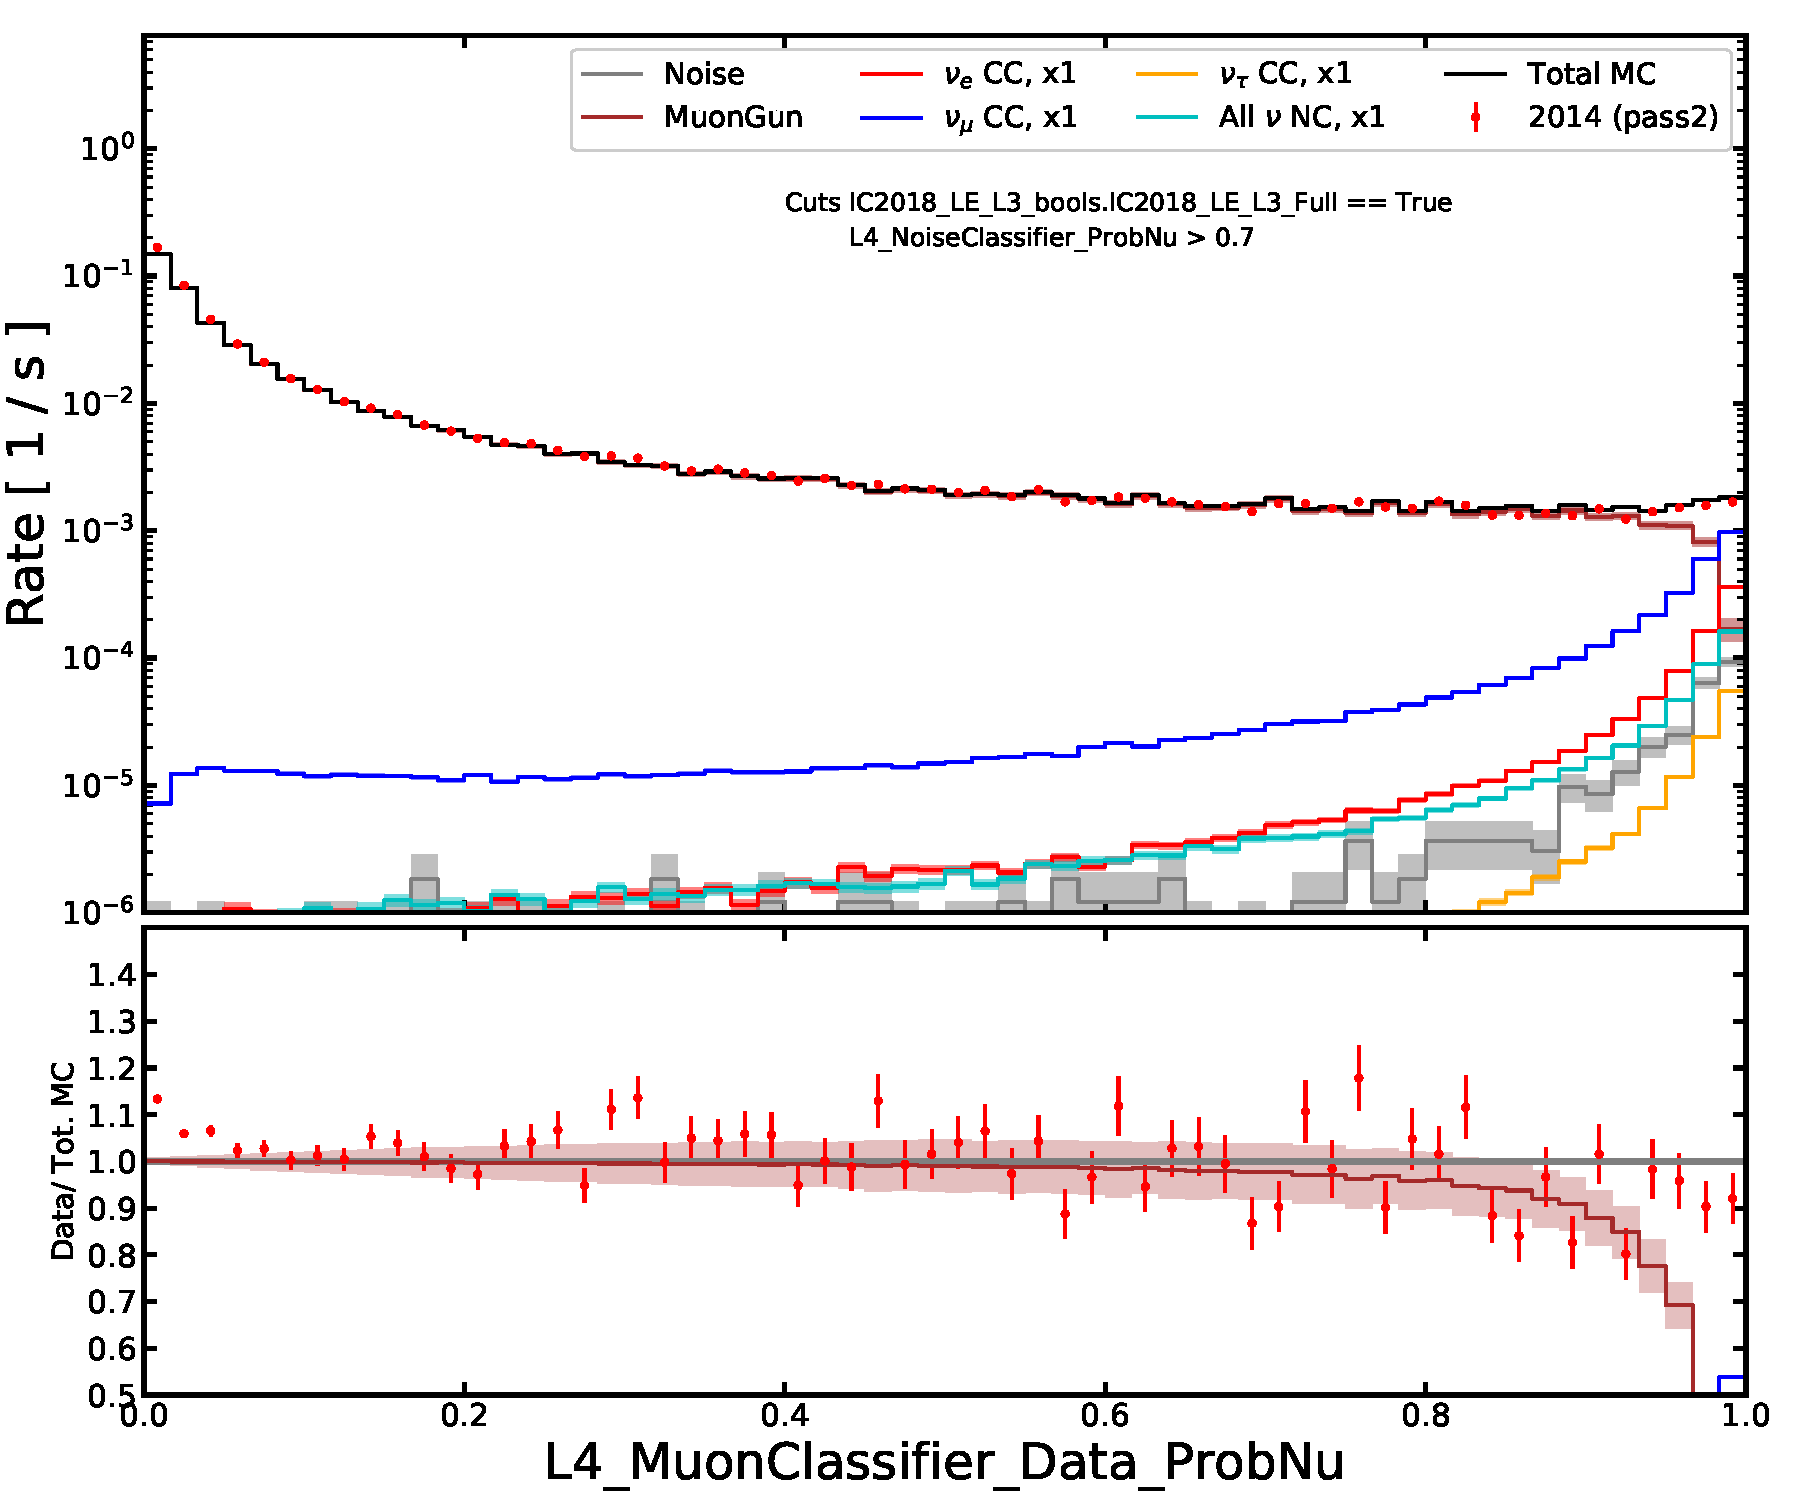
\includegraphics[width=7 cm]{figures/icecube/selection/L4_muon_L4_MuonClassifier_Data_ProbNu.pdf}
    \caption{Distribution scores for the noise (left) and muon (right) BDT. The distributions of the muon classifier are shown for events where the score of the noise BDT is greater than 0.7.}
    \label{fig:l4-bdt-output}
\end{figure*}

\subsubsection{Level 5}
The final offline filter level that is applied before the event reconstruction step is L5. This filter searches specifically for hits occurring in un-instrumented \emph{corridors} within the IceCube array through which an atmospheric muon can sneak into the DeepCore volume while evading previous veto cuts. In addition, events with more than seven hits in the outermost strings of the IceCube array or that have a down-going pattern of hits in the uppermost region of the detector are vetoed to remove events containing atmospheric muons entering the detector coincidentally with neutrinos. The distribution for one of the corridor variables and one of the muon rejection variables are shown in figure~\ref{fig:l5-vars}. Table~\ref{tab:l5_summary} shows the rates of each event type expected at each level of the selection up to L5 together with the efficiency of the filter at the final level.
\begin{figure*}
    \centering
    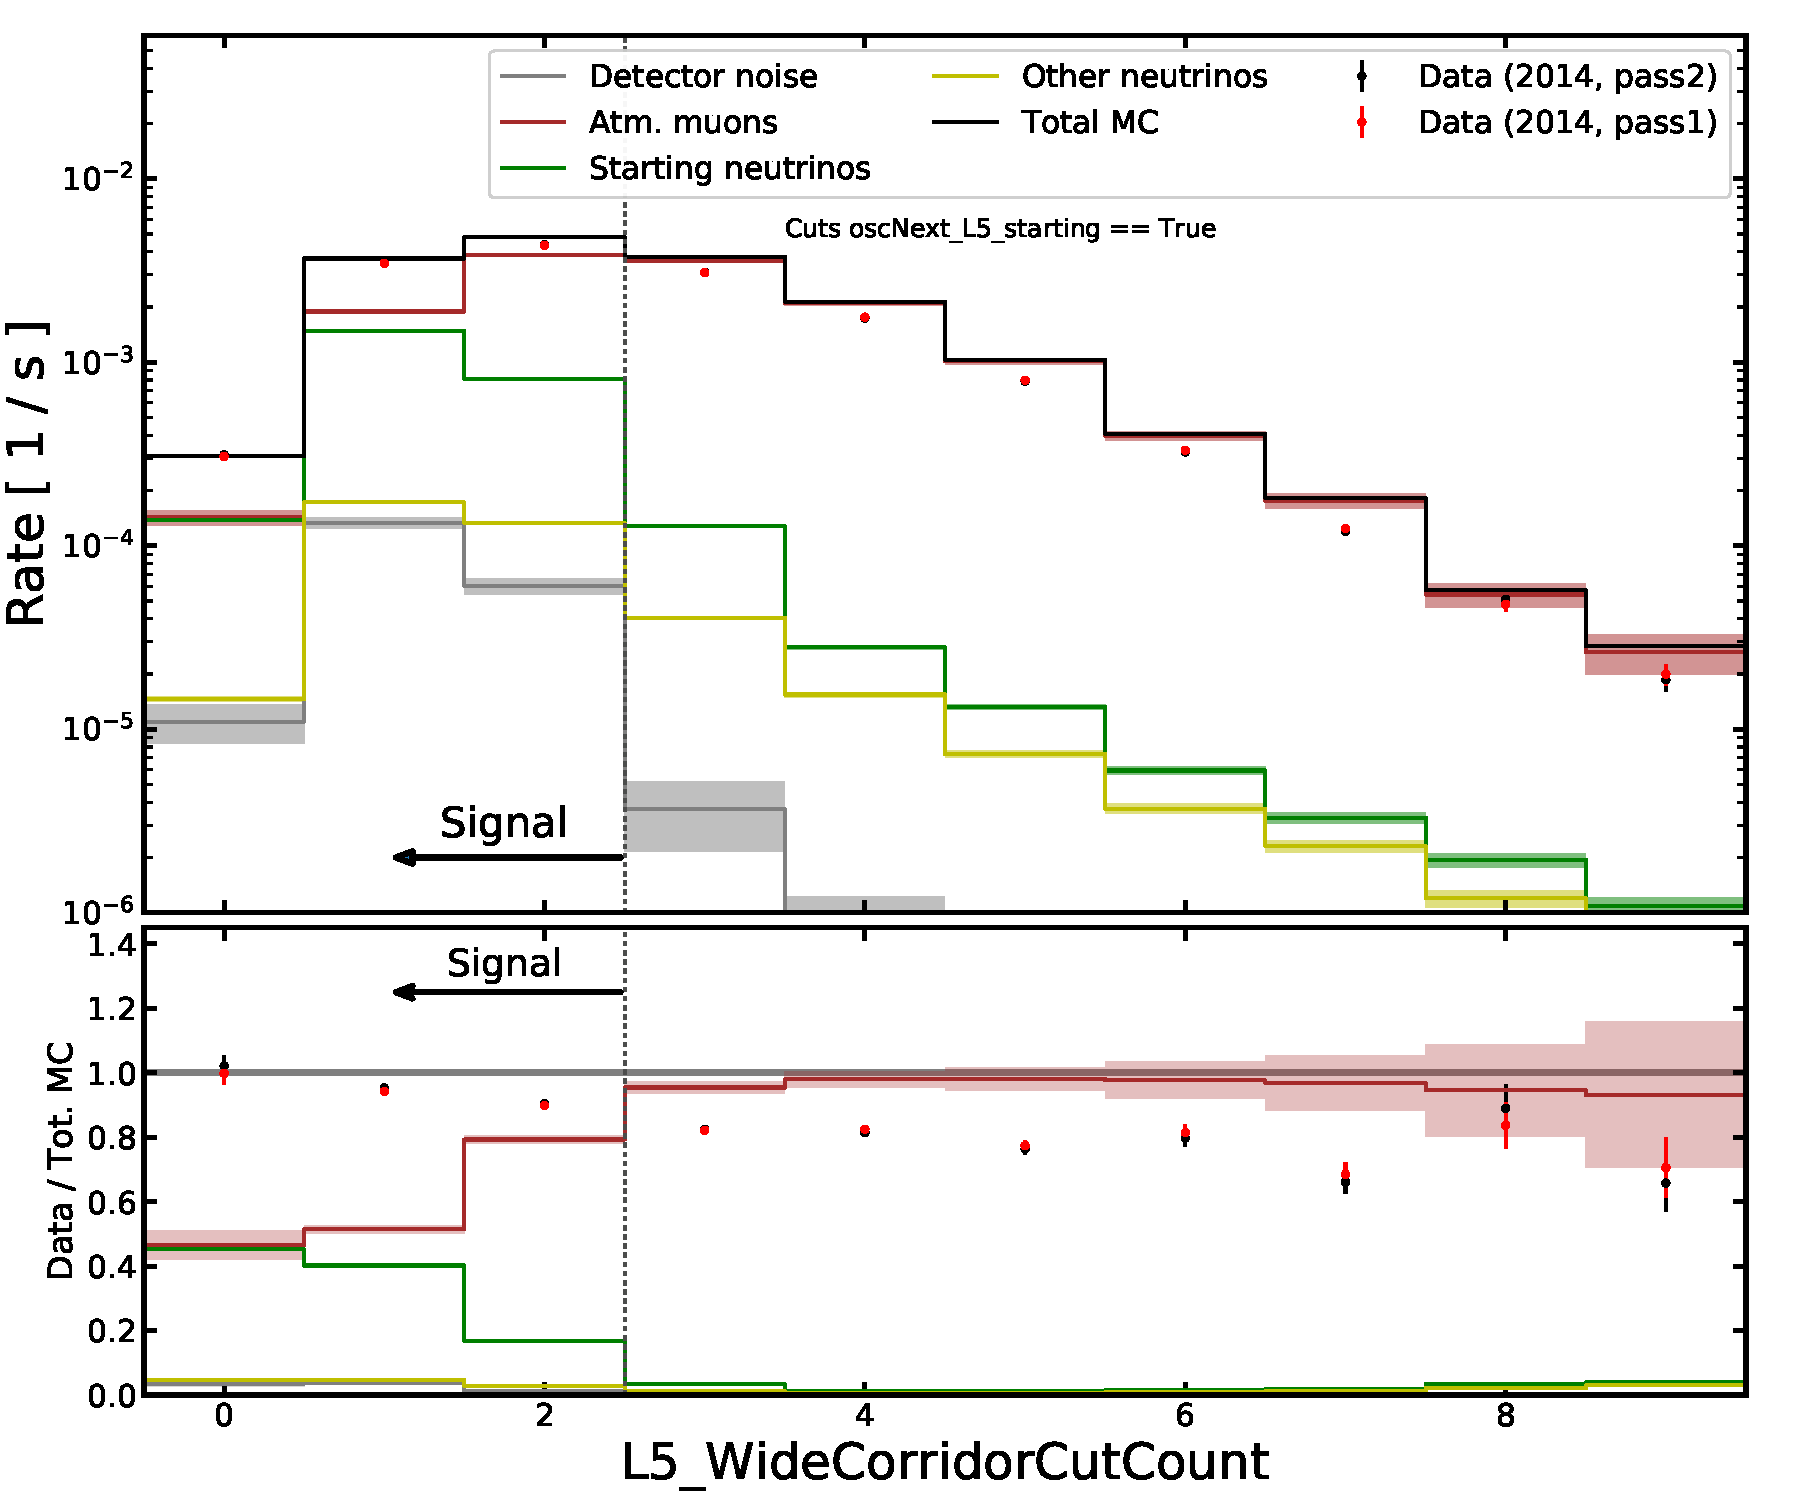
\includegraphics[width=7 cm]{figures/icecube/selection/L5_contained_L5_WideCorridorCutCount.pdf}
    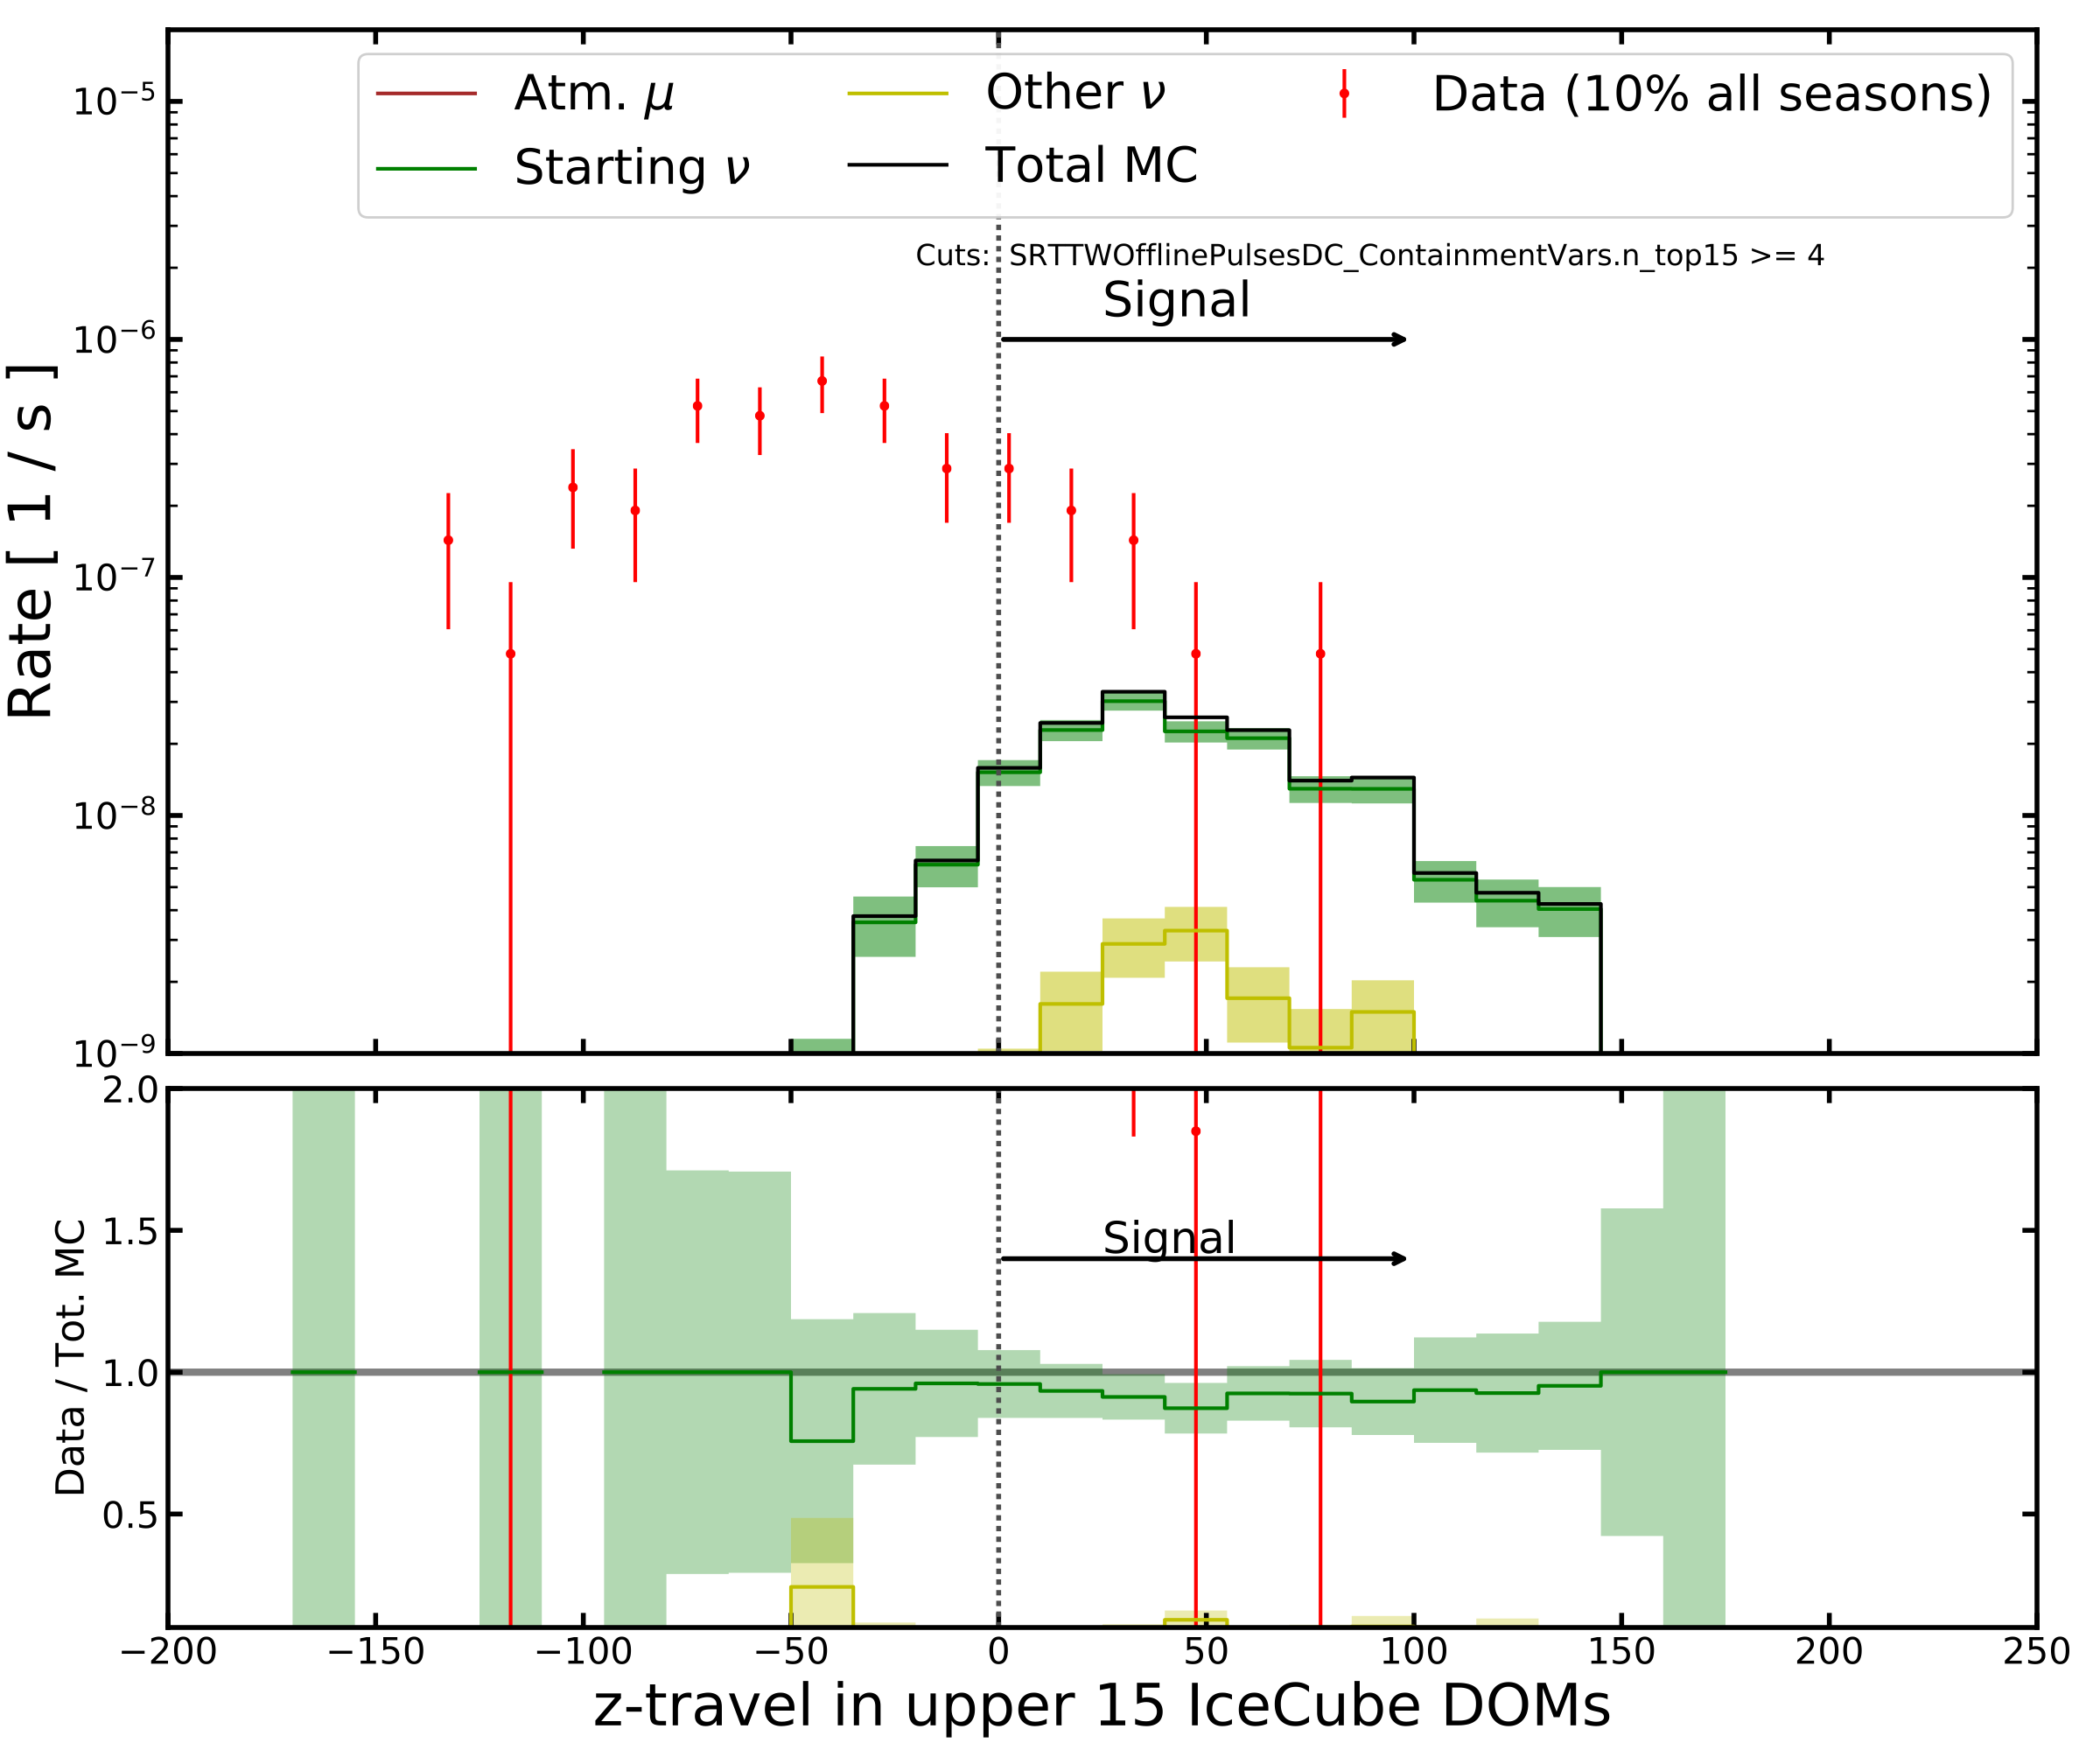
\includegraphics[width=7 cm]{figures/icecube/selection/SRTTWOfflinePulsesDC_ContainmentVars.z_travel_top15.png}
    \caption{Distributions for one of the L5 corridor cut variables (left) and one of the variables used to reject coincident muon events (right). The distribution in the right panel is shown only for events which have at least four hits in the uppermost 15 DOMs combined over all IceCube strings.}
    \label{fig:l5-vars}
\end{figure*}

\begin{table}
\begin{tabular}{lrrrrr}
Event type  & DC filter   & L3   & L4   & L5   & Eff. (\%) \\
\toprule
Atm. $\mu$         & 7273 & 505  & 28.1 & 0.93 & 0.012          \\
Pure noise         & 6621 & 36.6 & 0.28 & 0.07 & 0.001          \\
Atm. $\nu_e$ CC    & 1.61 & 0.95 & 0.84 & 0.48 & 29.8           \\
Atm. $\nu_\mu$ CC  & 6.16 & 3.77 & 3.11 & 1.39 & 22.5           \\
Atm. $\nu_\tau$ CC & 0.19 & 0.13 & 0.12 & 0.07 & 36.8           \\
Atm. $\nu$ NC      & 0.86 & 0.53 & 0.46 & 0.23 & 26.7  \\
\end{tabular}
\caption{Summary of the rates (in mHz) obtained after each level of selection. Neutrinos are weighted to an atmospheric spectrum with oscillations included.}
\label{tab:l5_summary}
\end{table}

\subsection{Event Reconstruction}
\label{sec:event-reconstruction}

After the L5 selection, the rate of muons is reduced enough such that the majority of the total sample is expected to consist of atmospheric neutrinos, and it is at this point that the event reconstruction and signature classification is run. For the measurement presented in this thesis, three reconstructed quantities are required: The zenith angle, the energy, and a proxy score that determines the flavor of a neutrino. As described in section \ref{sec:particle-signatures}, all neutrino events in DeepCore can be effectively approximated as either a cascade ($\nu_e$ CC events, all NC events, and 83\% of $\nu_\tau$ CC events) or a combination of a cascade at the neutrino interaction point with an out-going muon track ($\nu_\mu$ CC events and 17\% of $\nu_\tau$ CC events). The zenith angle can be most accurately reconstructed for track-like events due to their elongated, highly directional signature. For cascades, the reconstruction of the direction is more difficult because of their most compact and diffuse light distribution. The energy of a neutrino event is reconstructed by comparing the expected light output of a combined track and cascade hypothesis to the observed hits. Finally, the flavor proxy is calculated using variables that characterize the elongation of the observed hit signature  and the goodness-of-fit of a combined track and cascade hypothesis compared to that of a cascade-only hypothesis. The resulting score allows the separation of muon neutrino interactions from other interactions, which is ideally suitable to observe the muon neutrino disappearance oscillation channel.

\subsubsection{Zenith angle reconstruction}
The zenith is reconstructed using an old but refurbished algorithm that first removes hits from light that is likely to have undergone a significant amount of scattering and then runs a modified $\chi^2$ fit on the observation times of the remaining hits assuming that they all lie on a Cherenkov cone that would be produced by a minimally ionizing muon. Because of the required hit cleaning step, not all events present at L5 can be reconstructed in this way. However, those events that pass the cleaning condition are the cleanest, most track-like events of the entire sample and therefore can be seen as a high-quality "golden sample".

